\chapter{Introduction}
\label{cpt:introduction}

\section{Chip Multi Processor}

Moore's Law~\cite{Moore1998}, an observation made by G. E. Moore one of the co-founders of Intel, has been the driving force behind processor development since its beginning.
The law is simply an observation; that scaling of transistors used to make integrated circuits will allow for approximately twice the number of transistors per die every 18 month.
Up until the mid-2000s, manufacturers used these additional transistors to increase single-core performance.
To improve performance manufacturers increased the clock frequency, and they used the increasing number of transistors to make increasingly complex processor cores.
Features such as speculative and out-of-order execution were added to take advantage of instruction-level parallelism (ILP) present in computer programs.
By the mid-2000s, processor cores had become so complex and were running at a frequency so high that manufacturers had reached what could be called a power wall.
Manufacturers were unable to continue increasing frequency and the transistor count of each core without attaching high-performance cooling systems to counter the increase power usage and hence increase heat generation.
Systems like water or even nitrogen cooling were needed to continue the performance increase~\cite{Sutter2005}; these systems are not suitable for personal computers.

By 2005, most manufacturers had abandoned their plans for increased single core performance, and where all working towards chip multiprocessors (CMPs)~\cite{Sutter2005}.
Instead of the complex cores used in single core processors CMPs were built using simpler processing cores with less aggressive ILP utilization.
This allowed manufacturers to fit multiple cores on a single die, without hitting the power wall.
With an increasing number of transistors due to scaling, even more processing cores can be added to CMPs.
Today CMPs are the de-facto standard, being use in everything from embedded computers\todo{cite some arm, avr, etc spec} to commercial and high-performance computing~\cite{Thomadakis2011, Jain2013}.


\section{CMP Memory System}

\begin{figure}[ht]
\centering
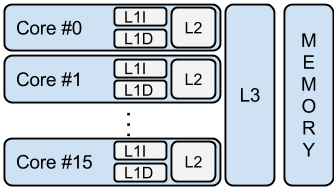
\includegraphics[scale=.5]{figures/processor_model/processor_model}
\caption{Generic Chip Multiprocessor Architecture}
\label{fig:cmp_model}
\end{figure}

Memory is a vital component of any computing system, without memory we are unable to store our programs and computations.
Traditionally the technology used to create memories have differed from the technology used in processors~\cite{Wilkes2001}.
As processor performance increased, memory performance did not increase proportionally.
This development has resulted in what is known as the processor-memory gap~\cite{Wilkes2001}.\todo{plot av gap}
In order to mitigate this effect, small and fast memory structures known as caches are a vital part of CMPs.
Any memory request issued by a processing core is filtered through one or multiple caches before being issued to the main memory.
If any of the caches has the value of the requested memory address, the value is returned, and the memory request never reaches the main memory.
This mechanism to an extent can hide the processor-memory gap, given a high hit rate in cache memories.

Traditionally there are three main ways of organizing cache memory; direct, set-associative and fully associative.
Caches used in commercial CMPs~\cite{Thomadakis2011, Jain2013} today are set associative memory structures.
A cache is organized a 2d array, where each row is called a set, and each set consist of one or more blocks.
A block, or a cache line, stores data from main memory.
The cache divides all memory addresses into three portions, the set address, block tag and block offset.
The set address is used to determine which set is responsible for caching this address.
Within a set, all blocks are valid cache locations.
Each block in use stores the block tag of the data it has stored, so a lookup will scan for a block with a block tag matching the block tag from the address.
For a direct mapped cache, each set contains only one block, making the block scan cheap.
Fully associative caches contain only a single set, hence making any block a valid cache location for any address, the block scan is expensive in this case.
Set associative caches, also known as n-way caches, is a middle ground organization that stores n blocks per set.
Figure~\todo{create} shows the three cache organizations and how each divides an incoming memory address during a lookup.
When a request for an address cannot be satisfied by a cache, the cache will send the request to the next level in the memory hierarchy.
Once the cache receives a response from the lower level, the data is stored to provide faster access time if the block is later referenced.
For a set-associative or fully associative cache, there are multiple valid storage positions.
An algorithm, known as a cache partitioning algorithm, defines how the new block is stored in the cache.
Whenever we reference a cache in the remainder of the thesis, a set associative cache is implied unless otherwise specified.

In the memory hierarchy, smaller means faster. 
For instance, main memory is much faster than disks, but disks can store much more data.
The same is valid for caches, a smaller cache has a lower response time compared to a larger cache.
Figure~\ref{fig:cmp_model} shows an example 16-core CMP architecture with three cache levels and main memory.
For each cache level, the size increased and response time decreases.
The first level caches are the smallest while the third level caches are largest.
In order to save area on CMP chips, and also to provide an easy mechanism for data sharing between cores, it is common to have one level of shared cache.
In figure~\ref{fig:cmp_model} each core has a private L1 and L2 cache, but the final L3 cache is shared among all cores.
While sharing cache can improve performance, and improve overall utilization, it also makes the memory system exposed to destructive interference that potentially can hurt the performance of all processing cores. 
It is the cache partitioning algorithms job to manage access to shared caches, and to a varying extent reduce interference.


\section{Requirements and Contributions}
By analyzing the problem description, as given in chapter~\ref{cpt:problem_decription}, we have been able to extract a set of requirements for this thesis:

\begin{description}
    \item[R1] Introduce CMPs, their memory system, and the role of a cache partitioning algorithm.
    \item[R2] Present important and recent work in the cache partitioning field. Present their strength and weaknesses, and compare them based on expected performance and overhead.
    \item[R3] Create a framework for evaluation of various cache partitioning algorithms.
    \item[R4] Implement at least one of the presented algorithm and compare against a conventional LRU-managed cache.
\end{description}

Based on the second requirement, this thesis will include a curated list of cache partitioning algorithms selected for their importance or recency in the field.
Due to the amount of work in this field we have to select some properties that each algorithm must have in order to appear in our list of algorithms.
Each algorithm will be presented in detail at a theoretical level, with comparisons to other relevant algorithms.

To fulfill the fourth requirement, we will implement a simulation framework and within that framework implement several of the algorithms selected.
We present a series of experiments executed on this implementation.
The resulting data will be used to compare the various algorithms against each other, providing depth to the previously theoretical comparison.
In addition evaluations of the implemented simulation framework will also be performed.
These evaluations will explore the validity of our results.
The implemented simulation framework will at the end of this thesis be made available to NTNU and the CARD~\ref{CARD2015} group for future research.

\section{Outline}

Chapter~\ref{cpt:introduction} introduces the thesis by putting it in a historical context and presenting the contributions made, fulfilling requirement \textbf{R1}.
Then, chapter~\ref{cpt:algorithms} presents a selection of cache partitioning algorithms and provides a theoretical comparison between them, fulfilling requirement \textbf{R2}.
Next, chapter~\ref{cpt:implementation} presents the subset of algorithms that we implement within our simulation framework.
Any assumptions or changes we have made compared to the theoretical description of the algorithm in chapter~\ref{cpt:algorithms} are presented here.
Chapter~\ref{cpt:methodology} contains a description of our simulation framework and explains all metrics we later use to evaluate our experiments, this fulfills requirement~\textbf{R3}.
Next, chapter~\ref{cpt:results} presents all experiments performed during the work with this thesis and evaluates their results. 
This includes a performance comparison of all implemented cache partitioning algorithms, fulfilling requirement \textbf{R4}.
Finally chapters~\ref{cpt:discussion} and~\{cpt:conclusion} contains a discussion of our results and a conclusion based on these. 
In addition, an overview of future work is given.